\section{Integrals on curves and surfaces}

\begin{motivating}
How do you calculate the length of this curve?
\end{motivating}

\fixthis{PICTURE}

\begin{motivating}
How do you calculate the surface area of a sphere?
\end{motivating}

\fixthis{PICTURE}

Observe that these sets have $3$-dim volume 0.  To calculate arclength or surface area, we will need to \fixthis{integrate over the appropriate region. }

\subsection{Integrals on curves}

\fixthis{recall}


\begin{definition}
    A \textbf{vector-valued function} is a function $\bm{r}(t): \R \to \R^n$, given by
    $$\bm{r}(t) = \langle x_1(t),x_2(t), \cdots x_n(t) \rangle$$
    
    where all of the $x_i(t) : \R \to \R$ are single-variable functions.
    
    $\bm{r}(t)$ is also called a \textbf{parametrization} (with \textbf{parameter} $t$).
    \end{definition}


    We should think of a vector-valued function $\bm{r}(t)$ as describing the motion of a particle in $\R^n$. 

    \begin{definition}
    The path traced out by a parametrization is called a \textbf{parametric curve}.
    \end{definition}

\begin{center}
        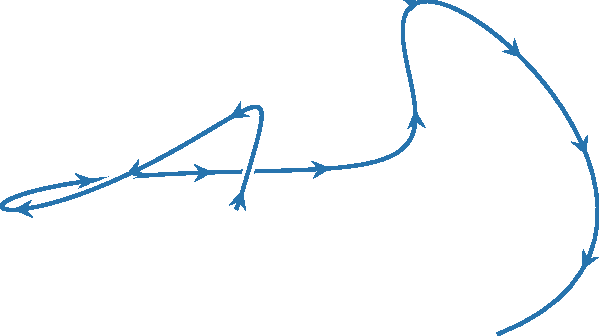
\includegraphics{chapters/5-IntegrationManifolds/figures/figures-paramcurve.pdf}
\end{center}

If a vector valued function $\bm{r}(t)$ describes the motion of an object in $\R^n$, how can we find the \textbf{distance} traveled by that object (from $t=a$ to $t=b$)?

\begin{definition}
    If $\bm{r}(t)$ models the motion of the object, the distance $D$ traveled (from $t=a$ to $t=b$) is given by the integral of the speed. That is, 
    $$D = \int_a^b ||\bm{r}'(t)|| \ dt$$ 
    \end{definition}

\begin{example}
Let $\bm{r}(t) = \langle \cos(t), \sin(t), 2 \rangle$ model the motion of a particle in $\R^3$. 
    
    Sketch the vector valued function, and find the distance traveled from $t=0$ to $t = 4\pi$.
\end{example}

How are your answers related to the parametric curve of $\bm{r}(t)$, and the length of the parametric curve?

\begin{definition}[]
    A \textbf{strict parametrization} of a curve $\mathcal{C} \subset \R^n$ is a vector-valued function $\bm{r}(t) : (a,b) \subset \R \to \mathcal{C}$ satisfying the following conditions:
    \begin{enumerate}    
        \item $\bm{r}(t)$ surjects onto $\mathcal{C}$.
        \item $\bm{r}(t)$ is injective for all $t \in (a,b)$.
        \item $\bm{r}(t)$ is differentiable.
        \item $\bm{r}'(t) \neq \bm{0}$ for all $t \in (a,b)$.    
    \end{enumerate}
    
    \end{definition}

     \begin{definition}[Arclength]
    Let $\mathcal{C}$ be a curve in $\R^n$, and let $\bm{r}(t) : (a,b) \to \R^n$ be a (strict) parametrization of $\mathcal{C}$.  
    
    Then the \textbf{arclength of $\mathcal{C}$} is defined to be the integral 
    
    $$\int_a^b ||\bm{r}'(t)|| \ dt$$
    
    \end{definition}

    \begin{example}
        Find the arc length of the vector-valued function $\bm{h}(t) = \langle -\sin(t), \cos(t), t \rangle$ from $t=0$ to $t=2\pi$.
    \end{example}

    \begin{definition}[Scalar line integral]
    Let $f : \R^n \to \R$ be a function of $n$ variables, and let $\mathcal{C}$ be a curve in $\R^n$.

    Let $\bm{r}(t) : (a,b) \to \R^n$ be a (strict) parametrization of $\mathcal{C}$.  Then the \textbf{scalar line integral  of $f$ over $\mathcal{C}$} is denoted $\int_\mathcal{C} f \ ds$, and is defined as the integral

    $$\int_\mathcal{C} f \ ds := \int_a^b f(\bm{r}(t)) \ ||\bm{r}'(t)|| \ dt$$
    
    \end{definition}

    \begin{center}
        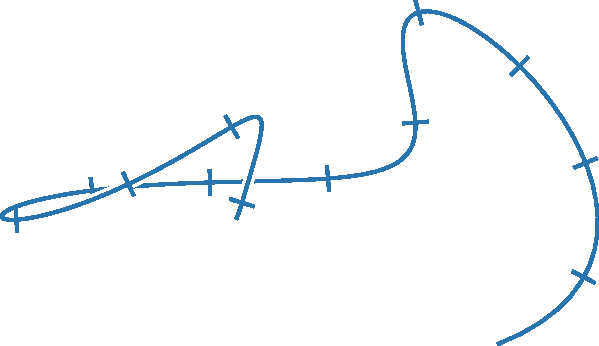
\includegraphics{chapters/5-IntegrationManifolds/figures/figures-partitioncurve.pdf}
    \end{center}

    \begin{example}
        Let $C$ be the helix, parametrized by $\bm{h}(t) = \langle -\sin(t), \cos(t), t \rangle$ for $0 \leq t \leq 3\pi$.  Calculate
    $$\int_C (x + y + z) \ ds$$
    \end{example}

    \begin{example}
     Find the total mass of a wire in the shape of a parabola $y = x^2$ for $1 \leq x \leq 4$ (in centimeters), with mass density given by $$\rho(x,y) = \frac{y}{x} \  \textnormal{grams/cm}$$   
    \end{example}

    \begin{motivating}
        Can you find a strict parametrization of the circle $x^2+y^2=1$ in $\R^2$?
    \end{motivating}

    Nope!

    \fixthis{recall}

    
    \begin{definition}
        Let $A \subset \R^n$.  We say that $A$ is an\textbf{ open subset of $\R^n$} if $A$ does not contain any of its boundary points.  That is, $$A \cap \partial A = \varnothing$$
    \end{definition}

     \begin{example}
        The interval $(a,b)$ is open in $\R$.  The sets $[a,b)$ and $[a,b]$ are \textbf{not open}.
    \end{example}

    \begin{example}
        The set $B_r(\bm{0}) := \{ \bm{v} \in \R^n \ | \ ||\bm{v}|| < 1\} $ is open in $\R^n$.  
    \end{example}

\begin{definition}[Parametrization]
    Let $\mathcal{C}$ be a curve in $\R^n$.  Let $A \subset \R$ be a subset such that $\textnormal{vol}_1(\partial A) = 0$.  Let $X \subset A$ be a subset such that $A - X$ is open.  Then  $\gamma : A \to \R^n$ is a \textbf{parametrization of} $\mathcal{C}$ if 
    
    \begin{enumerate}
        
        \item $\mathcal{C} \subset \gamma(A)$ (that is, $\gamma$ surjects onto $\mathcal{C}$).
        \item $\gamma(A - X) \subset \mathcal{C}$, and $\gamma : A - X \to \mathcal{C}$ is injective. 
        \item $\gamma(t)$ is differentiable for all $t \in A - X$.
        \item $\gamma'(t) \neq \bm{0}$ for all $t \in A - X$. 
        \item $\text{vol}_1(X) = 0$.
    \end{enumerate}
    
    \end{definition}

\begin{remark}
If $\gamma$ is a parametrization of $\mathcal{C}$, then $\gamma: (A-X) \to \mathcal{C} - \gamma(X)$ is a strict parametrization.
\end{remark}
    
\begin{example}
    Let $S^1$ be the circle $x^2+y^2=1$ in $\R^2$.
    
    Let $A = [0,2\pi] \subset \R$, and let $X = \{0, 2\pi\}$.  Then $A-X = (0,2\pi)$ is open, and $\text{vol}_1(X) = 0$.

    Let $\gamma(t) = \langle \cos(t) , \sin(t) \rangle$.


        \begin{enumerate}
        
        \item $S^1 = \gamma([0,2\pi])$.
        \item $\gamma(0,2\pi) \subset S^1$, and $\gamma : (0,2\pi) \to S^1$ is injective. 
        
        \item $\gamma'(t) = \langle -\sin(t), \cos(t) \rangle$.
        \item $\gamma'(t) \neq \bm{0}$ for all $t \in (0,2\pi)$.
    \end{enumerate}

    
    Therefore, $\gamma(t) = \langle \cos(t), \sin(t) \rangle$ parametrizes $S^1$:
    \end{example}

    \begin{definition}[Scalar line integral]
    Let $f : \R^n \to \R$ be a function of $n$ variables, and let $\mathcal{C}$ be a curve in $\R^n$.

    Let $\bm{r}(t) : (a,b) \to \R^n$ be a parametrization of $\mathcal{C}$.  Then the \textbf{scalar line integral  of $f$ over $\mathcal{C}$} is denoted $\int_\mathcal{C} f \ ds$, and is defined as the integral

    $$\int_\mathcal{C} f \ ds := \int_a^b f(\bm{r}(t)) \ ||\bm{r}'(t)|| \ dt$$
    \end{definition}


\subsection{Integrals on Surfaces in $\R^3$}

\begin{motivating}
    How do you calculate the surface area of a sphere?
\end{motivating}

\fixthis{picture}

\begin{definition}[]
    A \textbf{strict parametrization} of a surface $\mathcal{S} \subset \R^3$ is a multivariable function $G(u,v) : U \subset \R^2 \to \mathcal{S}$ satisfying the following conditions:
    \begin{enumerate}
        \item $U$ is an open set.
         
        \item $G(u,v)$ surjects onto $\mathcal{S}$.
        \item $G(u,v)$ is injective for all $\bm{u} \in U$.
     
        \item $G(u,v)$ is differentiable for all $\bm{u} \in U$ (that is, $\frac{\partial G}{\partial u}$ and $\frac{\partial G}{\partial v}$ exist).

        \item $[J_G(u,v)]$ is injective for all $\bm{u} \in U$.
    \end{enumerate}
    
    \end{definition}


\begin{theorem}
    The following statements are equivalent about a linear transformation $T : \R^n \to \R^m$ with standard matrix $A$:
    
    \begin{enumerate}
        \item $T$ is injective.
        \item The only solution to the equation $A\bm{x} = \bm{0}$ is $\bm{x} = \bm{0}$.
        \item If the equation $A\bm{x} = \bm{b}$ has a solution, it is unique.
        \item The columns of $A$ are linearly independent.
    \end{enumerate}
    
    \end{theorem}

\begin{example}
        Consider the surface $\mathcal{S}$ defined by $$\{(x,y,z) \ | \ x^2 + y^2 < 1, z=0\}$$ \fixthis{turn into polar rectangle}
        
        Let $U = \{(r,\theta) \ | \ 0 < r < 1, \ 0 < \theta < 2\pi\} \subset \R^2$, and let $$G(r,\theta) = \langle r\cos(\theta), r\sin(\theta), 0 \rangle$$

\begin{enumerate}               
        \item $G(u,v)$ surjects onto $\mathcal{S}$.
        \item $G(u,v)$ is injective for all $\bm{u} \in U$.
        
        \item $G(u,v)$ is differentiable for all $\bm{u} \in U$.

        \item $[J_G(u,v)]$ is injective for all $\bm{u} \in U$.
    \end{enumerate}

    So $G(r,\theta)$ is a strict parametrization of $\mathcal{S}$.
        
    \end{example}

    \begin{example}
        Consider the surface $\mathcal{S}$ defined by $$\{(x,y,z) \ | \ z= f(x,y), a < x < b, c < y < d\}$$

        Parametrize the surface $\mathcal{S}$.
    \end{example}


\begin{remark}
    Let $\mathcal{S}$ be a surface (strictly) parametrized by $G(u,v)$, and consider a point $P = G(u_0,v_0)$ on $S$.
    
    \vspace{1em}
    
    Observe that the functions $G(u,v_0)$ and $G(u_0,v)$ are curves on the surface $\mathcal{S}$ that intersect at $P$.
    \end{remark}
    
%    \begin{center}
%        \includegraphics[scale=0.4]{pictures/surfacetangent.png}
%    \end{center}

\begin{theorem}
    The tangent plane to $\mathcal{S}$ at a point $G(u_0,v_0)$ is spanned by the vectors $$\frac{\partial G}{\partial u}(u_0,v_0) = \left\langle \frac{\partial x}{\partial u}(u_0,v_0), \frac{\partial y}{\partial u}(u_0,v_0), \frac{\partial z}{\partial u}(u_0,v_0) \right\rangle$$
    $$\frac{\partial G}{\partial v}(u_0,v_0) = \left\langle \frac{\partial x}{\partial v}(u_0,v_0), \frac{\partial y}{\partial v}(u_0,v_0), \frac{\partial z}{\partial v}(u_0,v_0) \right\rangle$$
    \end{theorem}
    
    \begin{motivating}
        What is an equation for the tangent plane to $\mathcal{S}$ at a point $G(u_0,v_0)$?
    \end{motivating}
    
    \fixthis{recall}
\begin{theorem}
    Let $D$ be the parallelogram in $\R^3$ spanned by $\bm{u}$ and $\bm{v}$. Then
    $$\textnormal{area}(D) = ||\bm{u \times v}||$$
    \end{theorem}

\begin{theorem}
    Let $\mathcal{S}$ be a surface (strictly) parametrized by a function $\bm{\gamma} :  U \subset \R^{2} \to \R^3$.  Then the area of a parallelogram at a point $\gamma(\bm{u}) \in S$ is given by $$\textnormal{area}(D) = \left|\left|\frac{\partial \gamma}{\partial u}(\bm{u}) \times \frac{\partial \gamma}{\partial v}(\bm{u})\right|\right|$$ 
    \end{theorem}

\begin{definition}
    Let $\mathcal{S}$ be a surface (strictly) parametrized by a function $\bm{\gamma} :  U \subset \R^{2} \to \R^3$.  Then the \textbf{surface area of $\mathcal{S}$} is denoted by $\int_\mathcal{S} \ dA$, and defined to be
    $$\int_\mathcal{S} \ dS := \int_U \left|\left|\frac{\partial \gamma}{\partial u} \times \frac{\partial \gamma}{\partial v}\right|\right| \ dA$$
    \end{definition}

\begin{motivating}
    Can you find a strict parametrization of the sphere $x^2+y^2+z^2=1$ in $\R^3$?
\end{motivating}

\begin{definition}[Parametrization]
    Let $\mathcal{S} \subset \R^3$ be a surface.  Let $A \subset \R^2$ be a subset such that $\textnormal{vol}_2(\partial A) = 0$.  Let $X \subset A$ be a subset such that $A - X$ is open.  Then a map $\gamma : A \to \R^3$ parametrizes $\mathcal{S}$ if 
    
    \begin{enumerate}
        \item $\mathcal{S} \subset \gamma(A)$ (that is, $\gamma$ surjects onto $\mathcal{S}$).
        \item $\gamma(A - X) \subset \mathcal{S}$, and $\gamma : A - X \to \mathcal{S}$ is injective. 

        \item $\gamma$ is differentiable for all $\bm{u} \in A-X$   
        \item $[J_\gamma(\bm{u})]$ is injective for all $\bm{u} \in A - X$. 
        
        \item $\text{vol}_2(X) = 0$ and for any compact subset $C \subset \mathcal{S}$, $\text{vol}_2(\gamma(X) \cap C) = 0$.
    \end{enumerate}
    
    \end{definition}

\begin{definition}
    Let $X \subset \R^n$ be a bounded subset.  We say that $X$ has $k$\textbf{-dimensional volume 0} ($\textnormal{vol}_k(X) = 0$) if
    $$\lim_{N \to \infty} \sum_{\substack{C \in D_N(\R^n) \\ C \cap X \neq \varnothing}} \left(\frac{1}{2^N}\right)^k = 0$$
    
    \end{definition}
    

    
    \begin{definition}
    Let $X \subset \R^n$ be an arbitrary subset.  We say that $X$ has $k$\textbf{-dimensional volume 0} ($\textnormal{vol}_k(X) = 0$) if for all $R > 0$, $B_R(\bm{0}) \cap X$ has volume 0.
    
    \end{definition}

    \begin{example}
    Let $S^2$ be the sphere $x^2+y^2+z^2=1$ in $\R^3$.

\vspace{1em}

    Let $A = \{(\theta, \phi) \ | \ 0 \leq \theta \leq  2\pi, \ 0 \leq \phi \leq  \pi\} \subset \R^2$, and let $X = \partial A$.  Then $A-X$ is open, and $\text{vol}_2(X) = 0$.

    Let $\gamma(\theta, \phi) = \langle \cos(\theta)\sin(\phi), \sin(\theta)\sin(\phi), \cos(\phi) \rangle$.

    
        \begin{enumerate}
        
        \item $S^2 = \gamma(A)$.
        \item $\gamma(A-X) \subset S^2$, and $\gamma : (A-X) \to S^2$ is injective. 
        
        \item $[J_\gamma(\theta, \phi)] = 
\begin{bmatrix}
-\sin(\theta)\sin(\phi) & \cos(\theta)\cos(\phi) \\
\cos(\theta)\sin(\phi) & \sin(\theta)\cos(\phi) \\
0 & -\sin(\phi)
\end{bmatrix}$
    \end{enumerate}

    
    Therefore, $\gamma(\theta, \phi)$ parametrizes $S^2$.
    \end{example}

\begin{example}
    Calculate the surface area of sphere $S^2 \subset \R^3$.
\end{example}



\subsection{Exercises}

\begin{problem}{arclengthinR2}
    Let $f: \R \to \R$ be a differentiable function.  Find a formula for the arclength of the graph of $y = f(x)$ from $x=a$ to $x=b$.
\end{problem}

\begin{problem}{arclengthinpolar}
    Let $\langle r(t), \theta(t)\rangle$ be a parametrization of a curve in polar coordinates.  Find a formula for the arclength of the curve from $t=a$ to $t=b$.  (\textbf{Hint}: convert to rectangular coordinates).
\end{problem}

\begin{problem}{Bernoulli}
    The Bernoulli spiral has parametrization $\bm{r}(t) = \langle e^t\cos(4t), e^t\sin(4t) \rangle$.  Find the arclength of the Bernoulli spiral from the point $(1,0)$ to the point $(e^{\frac{\pi}{2}}, 0)$.
\end{problem}


\begin{problem}{helix1}
Let $C$ be the helix, parametrized by $\bm{r}(t) = \langle \cos(t), \sin(t), t \rangle$ for $0 \leq t \leq 3\pi$.  Calculate
    $$\int_C (x + y + z) \ ds$$
\end{problem}

\begin{problem}{line1}
Let $f(x,y,z) = ye^{z^2}$.  Compute $\int_C f \ ds$ for the piecewise linear path from $(0,0,1)$ to $(2,0,0)$ to $(1,1,1)$
\end{problem}

\begin{problem}{line2}
Let $C$ be the line segment from $(0,0,0)$ to $(6,2,2)$. Calculate $$\int_C x+yz \ ds$$
\end{problem}


\begin{problem}{paramcurve}
    Parametrize the curve $C$ in $\mathbb{R}^3$ formed by intersecting the cylinder $x^2 + y^2 = 1$ and the plane $x + y + z = 1$ in $\mathbb{R}^3$
\end{problem}

\begin{problem}{paramfunction}
    Find a parametrization of the graph of $f(x) = x^{\frac{1}{3}}$.
\end{problem}

\begin{problem}{paramreverse}
    Let $\bm{r}(t) : (a,b) \to \R^n$ be a parametrization of $\mathcal{C}$ from $\bm{r}(a) = P$ to $\bm{r}(b) = Q$.  Find a parametrization $\bm{s}(u)$ of $\mathcal{C}$ that starts at $Q$ and ends at $P$.

    \begin{subproblems}
    \item Can you use $\bm{s}(u)$ to calculate $\int_\mathcal{C} f \ ds$?
    \end{subproblems}
\end{problem}


\begin{problem}{param1}
 Find a compact region $D$ and a parametrization $\Phi : D \to \R^3$ that parametrizes the surface $S$ given as the set $\{(x,y,z) \ | \ z = x+y^2, \ 0 < x < y, \ 0 < y < 1 \}$.  Verify that $\Phi$ is a parametrization.
\end{problem}

\begin{problem}{surfaceint1}
    Let $S$ be the surface $\{(x,y,z) \ | \ z = x+y^2, \ 0 < x < y, \ 0 < y < 1 \}$.
    Compute the surface integral $\int_S (z-x) \ dA$.
\end{problem}

\begin{problem}{tangentplane}
    Let $S$ be a surface (strictly) parametrized by $G(u,v) = (u,v, f(u,v))$.  Find an equation for the tangent plane to $S$ at $P = G(u_0,v_0)$.
\end{problem}

\begin{problem}{surfaceareaplane}
    Find a parametrization of the plane $2x+y-z=2$, and find the area of the plane that lies below the triangle with vertices $(0,0,0)$, $(0,1,0)$, $(1,0,0)$.
    
\end{problem}

\begin{problem}{paramcone}
     Consider the cone defined by $M = \{(x,y,z) \ | \ x^2 + y^2 - z^2 = 0, \ 0 < z < 1\}$.  Find the regions $A$ and $X$ in $\R^2$ such that the map $\gamma(r,\theta) = \langle r\cos(\theta), r\sin(\theta), r$ is a parametrization of the cone.
\end{problem}

\begin{problem}{surfaceint2}
    Calculate the surface area of the cone defined by $M = \{(x,y,z) \ | \ x^2 + y^2 - z^2 = 0, \ 0 < z < 1\}$.
\end{problem}


\begin{problem}{paramsurface3}
     Show that $\gamma(u,v) = \langle u^2, uv, v^2 \rangle$ parametrizes the surface $M$ given by $xz-y^2 = 0$. 
\end{problem}

\begin{problem}
    Calculate $\int_S (z-x) \ dS$, where $S$ is the portion of the graph of $z = x + y^2$, where $0 \leq x \leq y$, $0 \leq y \leq 1$.
\end{problem}

\begin{problem}{sphereint}
    Let $S$ be the surface that is the portion of the sphere $x^2 + y^2 + z^2 = 4$ where $1 \leq y^2 + z^2 \leq 3$, $y \geq 0$, and $x \geq 0$. Compute the surface integral $$\int_S \frac{1}{x} \ dS$$
\end{problem}


\section{Manifolds}

    \begin{motivating}
    How do we calculate the $2$-dimensional volume of a surface in $\R^n$?
    \end{motivating}

    \begin{motivating}
    If curves are 1-dimensional objects, and surfaces are 2-dimensional objects, how do we generalize to $k$-dimensional objects?
    \end{motivating}

    \begin{motivating}
    How do we calculate the $k$-dimensional volume of a $k$-dimensional manifold in $\R^n$?
    \end{motivating}


\begin{definition}
    A subset $M \subset \R^n$ is a \textbf{differentiable $k$-dimensional manifold embedded in $\R^n$}  if:
    
    for all $\bm{x} \in M$, there exists an open neighborhood $U \subset \R^n$ such that $M \cap U$ is the graph of a $C^1$ mapping $f: \R^k \to \R^{n-k}$.
    
    \end{definition}

Often, we will simply say $M$ is a differentiable $k$-dimensional manifold, forgetting the embedding of $M$ in $\R^n$.  Indeed, manifolds are independent of this embedding (which is called a choice of coordinates).  See \Cref{mfdindependence} for more details.

\begin{example}
    The graph of a $C^1$ vector-valued function $\bm{r}(t) : \R \to \R^{n-1}$  is a differentiable curve in $\R^n$.
    \end{example}

\fixthis{PICTURE}

\begin{example}
    The graph of a $C^1$ function $f : \R^n \to \R$  is a differentiable $n$-manifold in $\R^{n+1}$.
    \end{example}

\begin{example}
    The circle $S^1 = \{(x,y) \ | \ x^2 + y^2 = 1\}$ is a differentiable 1-manifold in $\R^2$.
    \end{example}    

\begin{example}
    The sphere $S^2= \{(x,y,z) \ | \ x^2 + y^2 + z^2 = 1\}$ is a differentiable surface in $\R^3$.
    \end{example}

\begin{example}
    The open unit disk $D = \{(x,y) \ | \ x^2 + y^2 < 1 \}$ is a 2-manifold in $\R^2$. \textbf{What is the map?}
    \end{example}


\begin{example}
        If $m \neq k$, the graph of a differentiable function $f : \R^m  \to \R^{n}$  is \textbf{not} a differentiable $k$-dimensional manifold.
    \end{example}

\begin{example}
    The closed unit disk $D = \{(x,y) \ | \ x^2 + y^2 \leq 1 \}$ is \textbf{not} a manifold.
    \end{example}


    \begin{example}
    The graph of $f(x) = |x|$ in $\R^2$ is not a manifold.  
    \end{example}

    \begin{example}
   The grpah of the vector-valued function $\bm{r}(t) : \R \to \R^2$ defined by $$\bm{r}(t) =  \langle 2\cos(t), \frac{4}{3}\sin(2t) \rangle$$ is \textbf{not} a curve.
    \end{example}


\begin{motivating}
    How can we describe manifolds?  
\end{motivating}

\begin{definition}[Parametrization]
    Let $\mathcal{M} \subset \R^n$ be a $k$-dimensional manifold embedded in $\R^n$.  Let $A \subset \R^k$ be a subset such that $\textnormal{vol}_k(\partial A) = 0$.  Let $X \subset A$ be a subset such that $A - X$ is open.  Then a map $\gamma : A \to \R^n$ parametrizes $\mathcal{M}$ if 
    
    \begin{enumerate}
        \item $\mathcal{M} \subset \gamma(A)$ (that is, $\gamma$ surjects onto $\mathcal{M}$).
        \item $\gamma(A - X) \subset \mathcal{M}$, and $\gamma : A - X \to \mathcal{M}$ is injective. 

        \item $\gamma$ is differentiable for all $\bm{u} \in A-X$   
        \item $[J_\gamma(\bm{u})]$ is injective for all $\bm{u} \in A - X$. 
        
        \item $\text{vol}_k(X) = 0$ and for any compact subset $C \subset \mathcal{M}$, $\text{vol}_k(\gamma(X) \cap C) = 0$.
    \end{enumerate}
    \end{definition}

\begin{remark}
    Parametrizations make it easy to find points on and sketch manifolds, but it is hard to check if a given point is on the manifold.
    
    $$\bm{r}(t) =  \langle \cos^3(t) - 3\sin(t)\cos(t), t^2-t^5 \rangle$$
    \end{remark}




\subsection{Integration on Manifolds}

\begin{remark}
    If $M \subset \R^n$ is a differentiable $k$-manifold, then locally, $M$ looks like $\R^k$.  In other words, we can locally approximate $M$ by the graph of a linear map (e.g. a hyperplane).  
    \end{remark}
    
    
    
    
    \begin{remark}
    Thus, the volume of a differentiable $k$-manifold can be approximated by the volume of $k$-dimensional parallelpipeds in $\R^n$.
    \end{remark}

\begin{definition}

Recall that given an $T = [T_{i,j}] \in M_{n \times m}(\R)$, the \textbf{transpose matrix} $T^\top \subset  M_{m \times n}(\R)$ is given by $$T^\top = [T_{j,i}]$$
\end{definition}

\begin{theorem}
    Let $D$ be the $k$-dimesional parallelpiped spanned by $\bm{v_1}, \cdots, \bm{v_k}$ in $\R^k$.  Consider the $k \times k$ matrix $T$ given by 
        \begin{equation*}
T := \begin{bmatrix}
\bm{v_1} \cdots \bm{v_k}
\end{bmatrix}
\end{equation*}
    
    Then $$\textnormal{volume}(D) = | \textnormal{det} T | = 
     \sqrt{\det(T^\top T)}$$

    \end{theorem}

\begin{remark}
    Recall that the determinant is only defined on square matrices.  
    
    If we have $k$ vectors $\bm{v_1}, \cdots, \bm{v_k}$ in $\R^n$, then the matrix 
    \begin{equation*}
T := \begin{bmatrix}
\bm{v_1} \cdots \bm{v_k}
\end{bmatrix}
\end{equation*}
    
    is a  $k \times n$ matrix.  Thus $\det(T)$ is meaningless.  However, we can still calculate $\det(T^\top T)$!
    
    \end{remark}
    
    \begin{definition}
    Let $D$ be the $k$-dimesional parallelpiped spanned by $\bm{v_1}, \cdots, \bm{v_k}$ in $\R^n$.  Then $$\textnormal{volume}(D) = \sqrt{\det(T^\top T)}$$
    \end{definition}


    \begin{definition}[$k$-dimensional volume of a manifold]
Let $M \subset \R^n$ be a differentiable $k$-dimensional manifold, let $A \subset \R^k$ be a set with well-defined volume, and let $\gamma : A \to \R^n$ be a parametrization of $M$ (recall this includes $X \subset A$). 


Then we define the integral $\int_{\gamma(A-X)} dV$ to be the \textbf{$k$-dimensional volume of $M$}.
$$\int_{\gamma(A-X)} dV := \int_{A-X} \sqrt{\det([D\gamma(\bm{u})]^\top [D\gamma(\bm{u})])} \ dV$$

\end{definition}

\begin{definition}
Let $M \subset \R^n$ be a differentiable $k$-dimensional manifold, let $A \subset \R^k$ be a set with well-defined volume, and let $\gamma : A \to \R^n$ be a parametrization of $M$. 


Let $f : \R^n \to \R$ be a function.  We say $f$ is integrable over $M$ if the integral on the right hand side exists:
$$\int_{M} f \ dV := \int_{A-X} f (\gamma(u)) \ \sqrt{\det([D\gamma(\bm{u})]^\top [D\gamma(\bm{u})])} \ dV$$

\end{definition}

\begin{example}
    Let $R > r > 0$. Compute the surface area of a torus (obtained by taking a circle of radius $r$  in the $xz$-plane, centered at $(R,0,0)$ and revolving it about the $z$-axis.
\end{example}

















\subsection{Identifying manifolds}

\begin{motivating}
    How can we recognize manifolds?
\end{motivating}

It is difficult to prove that a particular set $X$ is a manifold using \Cref{mfddefn} - for every point in $X$, you must produce an open set $U$ and a $C^1$-map $f$ (such data is called an atlas).  In this class, we are most interested in when the set of solutions to a given equation is a manifold.  In this case, we can use multivariable calculus to identify manifolds!
    
    \begin{definition}
    Let $f : X \subset \R^n \to \R^m$ be a function. The \textbf{vanishing locus of $f$} (sometimes called the locus, or the zero locus) is the set of points $V(f)$ where $f$ vanishes.  That is, $$V(f) = \{\bm{x} \in X \ | f(\bm{x}) = 0 \} $$
    \end{definition}


   Parametrizations make it easy to find points on and sketch manifolds, but it is hard to check if a given point is on the manifold.  On the other hand, given a vanishing locus, it is easy to check if a given point is on the manifold, but it is difficult to find points on the manifold.  

    \begin{example}
        The unit circle $S^1 :=\{(x,y) \ | \ x^2 + y^2 = 1\}$ is a vanishing locus, and requires 4 open neighborhoods $U$ in $\R^2$ to show that it is a 1-dimensional manifold.
    \end{example}


    It turns out that we can use multivariable calculus to determine when a vanishing locus is a manifold!  Using a powerful theorem from analysis called the implicit function theorem, it turns out that locally (e.g. in a neighborhood $U$), we can identify a differentiable $k$-dimensional manifold embedded in $\R^n$ as the vanishing locus of a $C^1$-mapping $F : U \to \R^{n-k}$.  The key hypothesis that we need is that the derivative of $F$, $[J_F(\bm{z})]$ must be surjective.

    \begin{definition}
    A map $f : X \to Y$ is \textbf{surjective} if for every $y \in Y$, there exists an $x \in X$ such that $f(x) = y$.
    \end{definition}

    \begin{theorem}\label{surjectivity}
    The following statements are equivalent about a linear transformation $T : \R^n \to \R^m$ with standard matrix $A$:

    \begin{enumerate}
        \item $T$ is surjective.
        \item The columns of $A$ span $\R^m$.
        \item For every $\bm{b} \in \R^m$, there exists $\bm{x} \in \R^n$ such that $A\bm{x} = \bm{b}$.
        \item The rows of $A$ are linearly independent.
    \end{enumerate}
    \end{theorem}

    With this, we can now state local and global theorems that allow us to identify when a subset of $\R^n$ is a manifold:
    
    
    \begin{theorem}[Locally showing a vanishing locus is a differentiable manifold] \label{implicitlocal}
     Let $M$ be a subset of $\R^n$. Let $U \subset \R^n$ be open, and let $F : U \to \R^{n-k}$ be a $C^1$-mapping such that
    $$M \cap U = \{\bm{z} \in U \ | \ F(\bm{z}) = \bm{0} \}$$
    
    If the derivative $[J_F(\bm{z})]$ is a surjective map for every $\bm{z} \in M \cap U$, then $X \cap U$ is a differentiable $k$-dimensional manifold embedded in $\R^n$.  
    \end{theorem}


    
    \begin{theorem}[Showing a vanishing locus is a differentiable manifold] \label{implicitglobal}
    Let $M$ be a subset of $\R^n$.  If for every $\bm{z} \in M$, there exists an open set $U  \subset \R^n$ containing $\bm{z}$, and a $C^1$-mapping $F : U \subset \R^n \to \R^{n-k}$ such that 
    $$M \cap U = \{\bm{z} \in U \ | \ F(\bm{z}) = \bm{0} \}$$
    and $[J_F(\bm{z})]$ is surjective for every $\bm{z} \in M$, then $M$ is a differentiable $k$-dimensional manifold.
    \end{theorem}

    \begin{example}
        Unit circle
    \end{example}

One might be interested in the converse statement - can a differentiable manifold always be realized as a vanishing locus?  The answer is that this is always true locally (though not necessarily globally).

    \begin{theorem}[A differentiable manifold is locally a vanishing locus] \label{manifoldimplicit}
    Let $M \subset \R^n$ be differentiable $k$-dimensional manifold.  Then every point $\bm{z} \in M$ has a neighborhood $U \subset \R^n$ such that there exists a $C^1$-mapping $F : U \to \R^{n-k}$ such that $[J_F(\bm{z})]$ is surjective, and
    $$M \cap U = \{\bm{z} \in U \ | \ F(\bm{z}) = \bm{0} \}$$
    
    \end{theorem}
    
    \begin{remark}
    The $F$ in \Cref{manifoldimplicit} is not unique.  Therefore, we cannot use \Cref{implicitlocal} and \Cref{manifoldimplicit} to show that the locus defined by $F(\bm{z}) = \bm{0}$ is \textbf{not} a differentiable $k$-dimensional manifold.  In other words, the locus defined by $F(\bm{z}) = \bm{0}$ can be a differentiable manifold, even if $[J_F(\bm{z})]$ is \textbf{not} surjective. 
    \end{remark}

    \begin{example}
        Consider the function $F(x,y) = (x^2 + y^2 - 1)^2$.  
    \end{example}


This is a special case of the following theorem:

\begin{theorem}[Inverse image of a manifold]
Let $M \subset \R^m$ be a differentiable $k$-dimensional manifold embedded in $\R^m$.   Let $U \subset \R^n$ be open, and let $f : U \to \R^{m}$ be a $C^1$-mapping.
Let $f^{-1}(M)$ be the inverse image of $M$, 
$$f^{-1}(M) := \{\bm{x} \in \R^n \ | \ f(\bm{x}) \in M \}$$

If the derivative $[J_f(\bm{x})]$ is a surjective map for every $\bm{x} \in f^{-1}(M) \subset \R^n$, then $f^{-1}(M)$ is a differentiable $k + n - m$-dimensional manifold embedded in $\R^n$.
\end{theorem}

In our definition of a manifold, we had to explicitly choose coordinates by identifying which variables in $\R^n$ were the independent variables, and which were the dependent variables.  Thus our choices depended on the basis of $\R^n$.  In particular, it's not obvious that rotations of differentiable manifolds are still differentiable manifolds.

However, the choice of coordinates turns out to be unnecessary, and indeed, manifolds can be defined without referring to coordinates at all.

\begin{corollary}[Independence of coordinates]\label{mfdindependence}
Let $g : \R^n \to \R^n$ be a mapping of the form $$g(\bm{x}) = A\bm{x} + \bm{c}$$
where $A \in M_{n \times n}(\R)$ is an invertible $n \times n$ matrix.  If $M$ is a differentiable $k$-dimensional manifold, then $g(M)$ is also a differentiable $k$-dimensional manifold.
\end{corollary}









\subsection{Exercises}

\begin{problem}{nondiffcurve}
    Show that the graph of $f(x) = x^{\frac{1}{3}}$ is a differentiable 1-manifold (e.g. curve).
\end{problem}

\begin{problem}{params3}
    Find a parametrization of unit $3$-sphere in $\R^{4}$.  That is, $S^3 := \{(x,y,z,w) \in \R^4 \ | \ x^2+y^2 + z^2 + w^2 = 1\}$. (\textbf{Hint:} Generalize spherical coordinates!) 
\end{problem}

\begin{problem}{s3integral}
   Calculate $\int_{S^3} \ dS$ (that is, the 3-dimensional volume of $S^3$). 
\end{problem}

\begin{problem}{nsphere}
    Show that the $n$-sphere (defined by $\sum_{i=1}^n x_i^2 = 1$) is a differentiable $n-1$ manifold.
\end{problem}

\begin{problem}{vanishinglocussquared}
    Suppose that there exists a $C^1$-mapping $F : U \to \R^{n-k}$ such that $F(\bm{z}) = \bm{0}$ defines a manifold.  
\begin{enumerate}[label=(\alph*)]
    \item Show that $(F(\bm{z}))^2 = \bm{0}$ defines the same manifold.
    \item Show that $[J_F(\bm{z})]$ is never surjective.
\end{enumerate}
\end{problem}

\begin{problem}{vanishing locus manifold}
    For what values of $c$ is the locus of the equation $x^4+y^4+x^2-y^2 =c$ a differentiable manifold?
\end{problem}

\begin{problem}{tangentspacecircle}
    Use the three ways we saw in class to describe the tangent space of the unit circle.
\end{problem}

\begin{problem}{tangentspacesphere}
    Use the three ways we saw in class to describe the tangent space of the unit sphere.
\end{problem}

\begin{problem}{sl2}
    Consider $M_{2 \times 2}(\R)$, the set of $2 \times 2$ matrices with real entries.  Recall that $M_{2 \times 2}(\R) \cong \R^4$.

    Show that the set $$SL_2(\R) := \{ M \in M_{2 \times 2}(\R) \ | \ \textnormal{det}(M) = 1  \}$$ is a differentiable manifold in $\R^4$.  What is its dimension?
\end{problem}

\begin{problem}{gl2}
    Show that the set $$GL_2(\R) := \{ M \in M_{2 \times 2}(\R) \ | \ \textnormal{det}(M) \neq 0  \}$$ is a differentiable manifold in $\R^4$.  What is its dimension? (\textbf{Hint:} Use the inverse image of a manifold theorem).
\end{problem}

\begin{problem}{sinlines}
    For what values of $c$ is the vanishing locus of $f(x,y) = \sin(x+y) - c$ a differentiable manifold? 
    Describe and draw the vanishing locus of $f(x,y) = \sin(x+y) - 1$. 
\end{problem}